\documentclass{article}

% if you need to pass options to natbib, use, e.g.:
% \PassOptionsToPackage{numbers, compress}{natbib}
% before loading nips_2016
%
% to avoid loading the natbib package, add option nonatbib:
% \usepackage[nonatbib]{nips_2016}

%\usepackage{nips_2016}

% to compile a camera-ready version, add the [final] option, e.g.:
\usepackage[final,nonatbib]{nips_2016}

\usepackage[utf8]{inputenc} % allow utf-8 input
\usepackage[T1]{fontenc}    % use 8-bit T1 fonts
\usepackage{hyperref}       % hyperlinks
\usepackage{url}            % simple URL typesetting
\usepackage{booktabs}       % professional-quality tables
\usepackage{amsfonts}       % blackboard math symbols
\usepackage{nicefrac}       % compact symbols for 1/2, etc.
\usepackage{microtype}      % microtypography

\usepackage{graphicx}
%\setcitestyle{numbers}

\newcommand{\RR}{I\!\!R} %real numbers
\newcommand{\Nat}{I\!\!N} %natural numbers
\newcommand{\CC}{I\!\!\!\!C} %complex numbers

\title{Deep Models for Ensemble Touch-Screen Improvisation}

% The \author macro works with any number of authors. There are two
% commands used to separate the names and addresses of multiple
% authors: \And and \AND.
%
% Using \And between authors leaves it to LaTeX to determine where to
% break the lines. Using \AND forces a line break at that point. So,
% if LaTeX puts 3 of 4 authors names on the first line, and the last
% on the second line, try using \AND instead of \And before the third
% author name.

\author{
  Charles P. Martin\thanks{\url{http://charlesmartin.com.au}}\\
  Department of Informatics\\
  University of Oslo\\
  Norway\\
  \texttt{charlepm@ifi.uio.no}\\
  \And
  Kai Olav Ellefsen \\
  Department of Informatics\\
  University of Oslo\\
  Norway\\
  \texttt{kaiolae@ifi.uio.no}\\
  \And
  Jim T{\o}rresen\\
  Department of Informatics\\
  University of Oslo\\
  Norway\\
  \texttt{jimtoer@ifi.uio.no}\\
}

\begin{document}

\maketitle

\begin{abstract}
  For many, the pursuit and enjoyment of musical performance goes
  hand-in-hand with collaborative creativity, whether in an choir,
  jazz combo, orchestra, or rock band. However, few musical interfaces
  use the affordances of computers to create or enhance ensemble
  musical experiences. One possibility for such a system would be to
  use an artificial neural network to model the way other musicians
  respond to single performer. Some forms of music have
  well-understood rules for interaction; however, this is not the case
  for free improvisation with new touch-screen instruments where
  styles of interaction may be discovered in each new performance.
  This paper describes work-in-progress towards an ANN model of
  ensemble interactions that took place in such performances.
  Potential models have been trained on a corpus of ensemble
  touch-screen improvisations that has been made available from
  previous work. The results show realistic ensemble interactions that
  warrant further exploration.
\end{abstract}

\section{Introduction}

The proliferation of touch-screen enabled devices over the past decade
has resulted many creative digital musical instrument designs. One
appealing aspect of these devices is that they are often portable and
suggest use while among friends rather than in the office cubicle.
Several researchers have explored how these devices can be used in
ensemble situations such as Wang et al.'s ``MoPho'' mobile phone
orchestra~\cite{Wang:2014cs}, Schiemer's ``Pocket Gamelan''
works~\cite{Greg-Schiemer:2007mz}, and Snyder's marching band of DIY
mobile device powered instruments~\cite{Snyder:2014dp}. These works
demonstrate the very wide creative space of mobile computer music with
resulting applications frequently appealing to non-expert users as
well~\cite{Wang:2014ul, Hamilton:2011aa}.

In previous research, Martin et al.~\cite{Martin:2016rm} captured a
relatively large (for the field) dataset of more than 150
collaborative performances on mobile instruments as part of a project
exploring the design and impact of networked mobile music interfaces.
This dataset included both raw touch-data and time series of
interpreted touch-gestures sampled at a fixed interval. In the present
research, we suggest that this dataset could be used to train an
artificial neural network (ANN) that imitates the behaviour of the
ensemble based on the input of one user. While such a network may
allow us to understand more about the structure of interaction, we
envisage that it could be applied in practice as part of a system to
automatically accompany individual users of a mobile music app, thus
extending the experience of collaborative creativity to users and
situations where a live performance would not be possible.

Many improvised styles (e.g., jazz), have ensemble interactions based
on well-defined rules. Machine learning systems such as the
\emph{Reflexive Looper}\cite{Pachet:2013kq} and
\emph{SongSmith}~\cite{Morris:2008qe} take advantage of these rules to
create appropriate accompaniments. In the present research, the
improvised performances were ``free'', that is, performers were
allowed to perform in any way they wished within the constraints of
the touch-screen instruments. While it is clear that the performances
contained interaction between players, it is not clear how this
occurred. Thus prediction of this interaction can only be learned from
the data, without assistance from music theory.

It has previously been shown that long short-term memory (LSTM)
recurrent neural networks (RNNs) can be used for composing blues
music~\cite{Eck:2007rw}, folk tunes~\cite{Sturm:2016rz}, as well as
polyphonic music~\cite{Walder:2016le}. These networks have not, so
far, been applied to free-form improvised music using new interfaces
such as touch-screens. In this work, we show that such networks could
be practical for learning and generating the free-improvised ensemble
responses to a single lead player of a gestural touch-screen
interface.

\subsection{Interpreting Touch Data}

\begin{figure}
  \centering
  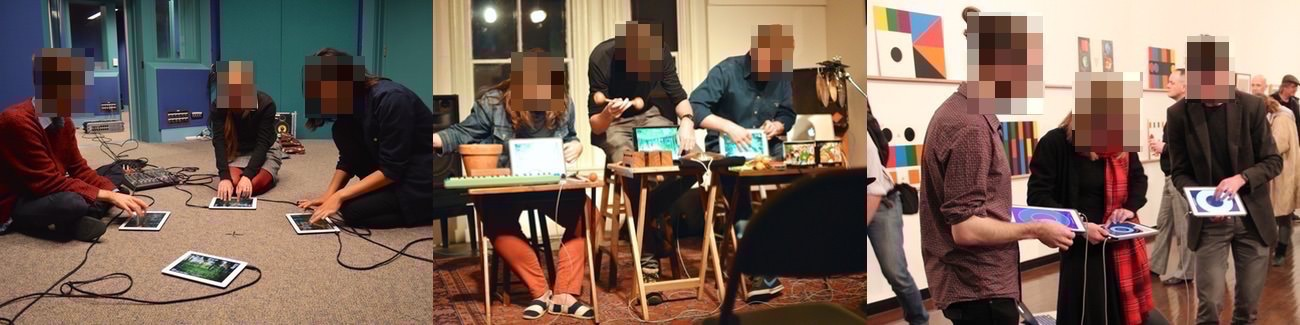
\includegraphics[width=0.9\textwidth]{three-performance-contexts}
  \caption{In previous work, data was collected from more than 150
    collaborative interaction sessions including rehearsals,
    performances, installations, and demonstrations. This corpus
    constitutes a significant dataset for investigations of
    creative interaction.}\label{fig:performance-contexts}
\end{figure}

Collaborative touch-screen interaction data was obtained from a
publicly-available corpus of collaborative touch-screen
performances~\cite{Martin:2016fc}. This corpus includes data from more
than 150 performances that included rehearsals, performances,
installations, and demonstrations. For the present research, only
ensemble improvisations were required, so data from demonstration
sessions and performances of composed works were removed. The
remaining data consisted of 72 improvised ensemble performances with a
total time of 9.8 hours.

Previous work has defined a method for interpreting raw touch
information (i.e., the time and location of taps and swipes) as a
sequence of continuous touch gestures~\cite{Martin:2015jk}. The
resulting sequences can be analysed to examine the structure of
performances. While the corpus contains touch data as well as these
interpreted touch-gestures, only the gestures will be considered in
the rest of this paper.

Working with this high-level data has advantages and disadvantages.
The state space is small (there are only 9 gestures in the vocabulary)
and these are sampled at a regular rate (1Hz) which reduces the
complexity of the data. Plots of these gesture sequences resemble
graphical scores and changes in performance style across the ensemble
can be seen at a glance. The gesture sequences, however, do not have a
one-to-one mapping with interaction in the app (e.g., tapping in any
part of the screen could be interpreted as the ``slow taps'' gesture)
so if sequences are generated automatically, they cannot be sonified
without further interpretation.

\section{ANN Model for Ensemble Performances}

To explore the potential for generating ensemble performances with
ANNs, multiple networks were trained corresponding to different
ensemble situations. In the following sections, each network will be
described and the results will be subjected to a preliminary
evaluation. Each network uses the same architecture of a recurrent
neural network (RNN) with long short-term memory (LSTM) cells. The
architecture of the networks mirrors the \emph{folkRNN} system
described by Sturm et al.~\cite{Sturm:2016rz} and consist of three
layers of 512 LSTM cells followed by a fully-connected softmax
layer\footnote{The TensorFlow implementation was aided by the blog
  posts of \emph{R2RT}\cite{R2RT-RNN:2016}}. In each case, the
networks were trained with minibatches of 64 performance examples each
consisting of 120 time-steps. Each of these examples corresponds to a
2-minute excerpt of a real collaborative performance. The networks
were implemented in TensorFlow~\cite{Abadi:2016wd} and were trained on
an Nvidia GeForce GTX 1080 GPU.

\subsection{Representing Ensemble Behaviour}

As previously mentioned, the goal of this work is to generate an
ensemble score based on the real improvisation of one player. To
achieve this, the ANNs were trained to the states of the ensemble
given the current lead player's state, and the state of the ensemble
at the previous time step. This arrangement is illustrated in Figure
\ref{fig:nn-ensemble-training}. As the training data consisted of
completely free improvisations, any player could be taken as the lead
so several training examples could be generated from a single slice of
a performance.

\begin{figure}
  \centering
  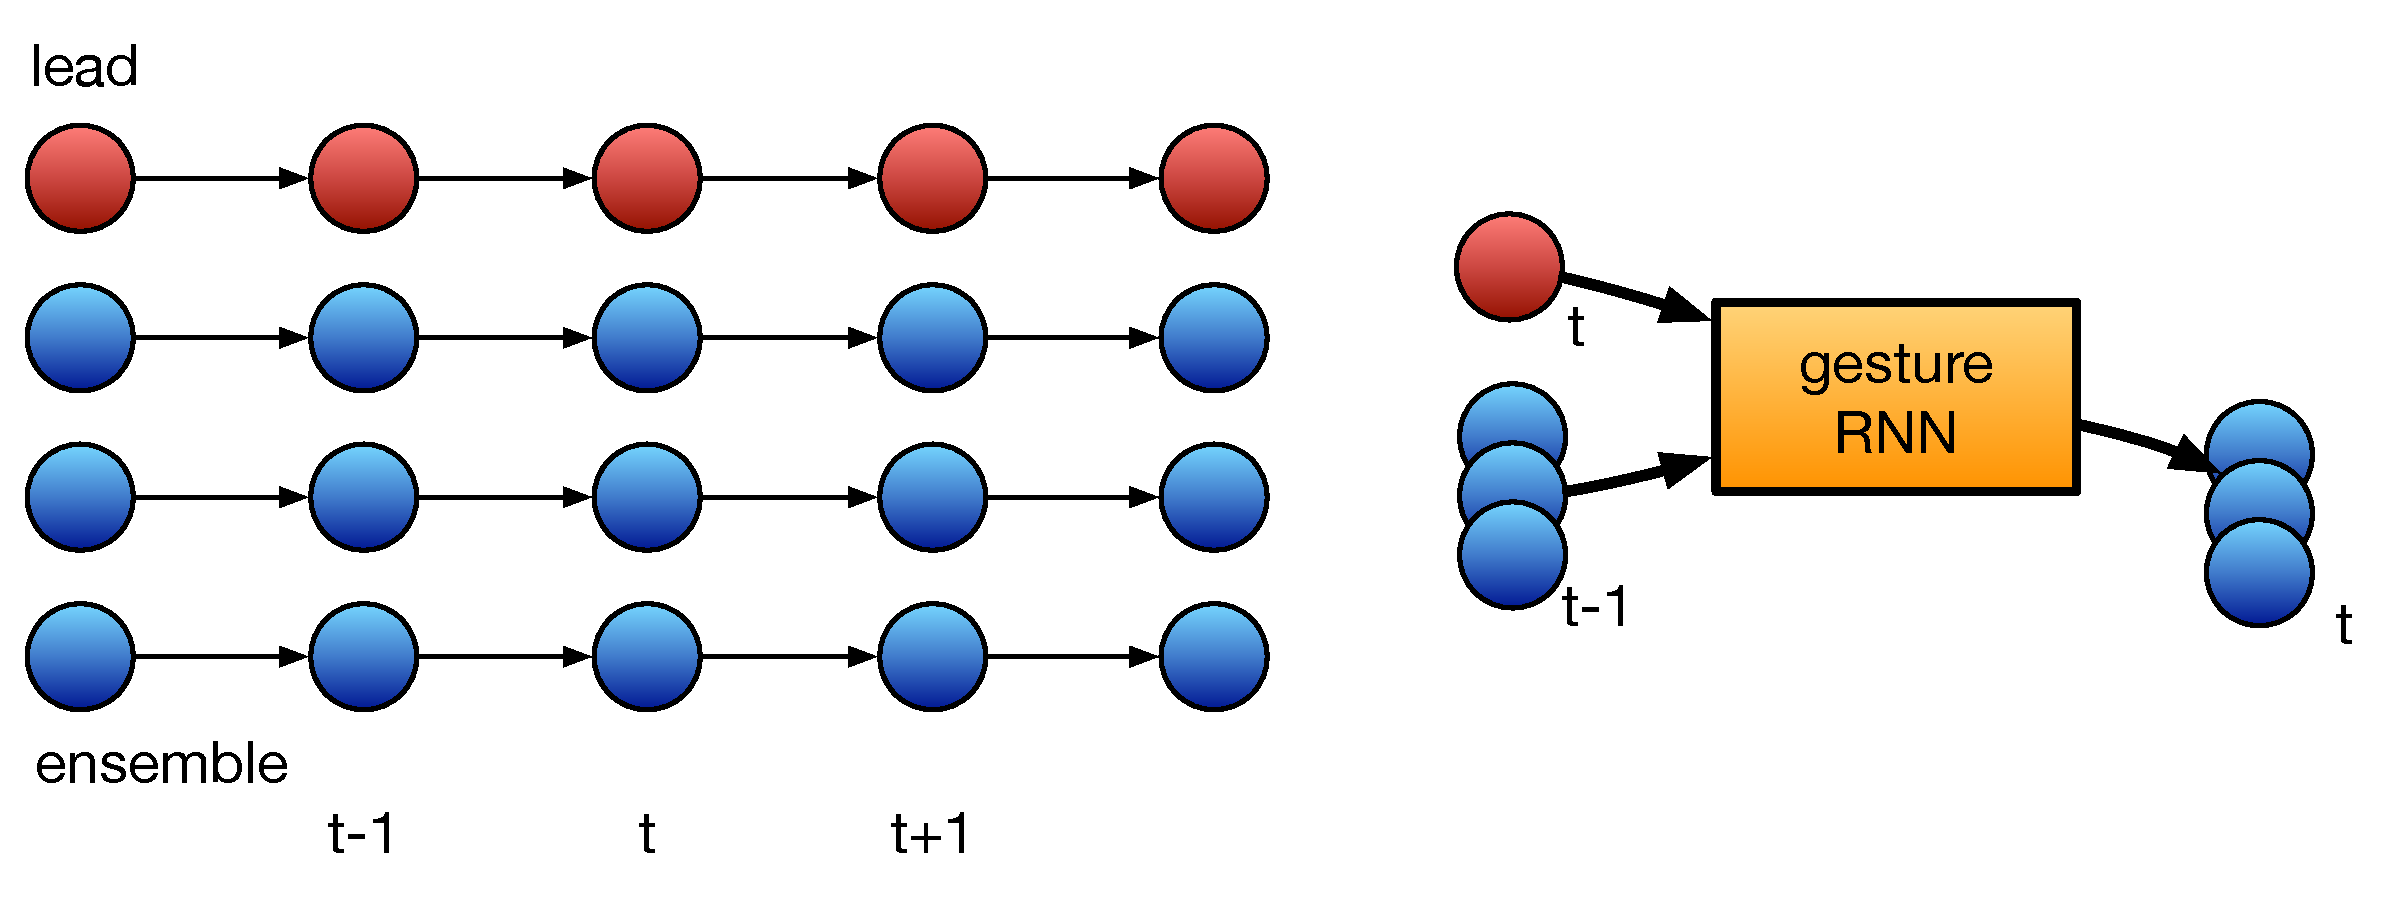
\includegraphics[width=0.8\textwidth]{nn-ensemble-training}
  \caption{The RNN was trained to predict a the ensemble states given
    the current lead state and previous ensemble
    states.}\label{fig:nn-ensemble-training}
\end{figure}

% \subsection{Individual Performers}

% Previous work has shown that LSTM networks can produce good results
% when generating musical and other sequences of data. A simple test for
% an LSTM network was to generate performance sequences of single
% players. This process could be repeated to generate multiple
% performances as shown in Figure \ref{fig:independent-model-test}.
% While the individual sequences are realistic, this is not an
% ``ensemble'' performance as the sequences are generated independently.
 
% % \begin{figure}
% %   \centering
% %   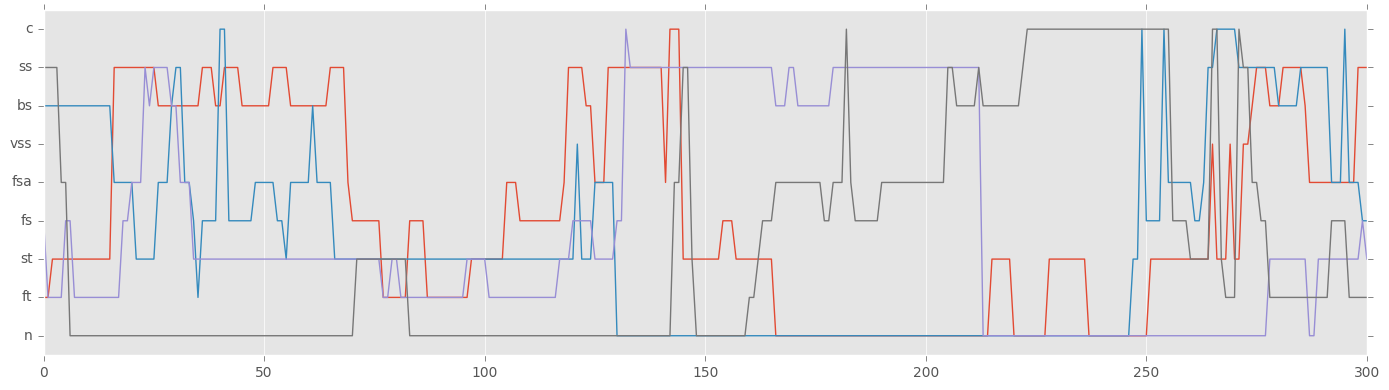
\includegraphics[width=\textwidth]{independent-networks-quartet}
% %   \caption{Four independently produced gesture sequences generated by
% %     the LSTM network. These sequences are realistic in their
% %     complexity, however, they are independent produced so do not show
% %     meaningful ensemble interaction.}\label{fig:independent-model-test}
% % \end{figure}

% A true ensemble model needs to encode not only the behaviour of single
% performers but how others in the group react to this behaviour.

%\subsection{One-hot ensemble representation}

In the dataset, each performer's actions are represented by one of
nine touch-gestures (including ``nothing''). We define a simple
encoding $\mathbb{N}_{<9}^n \rightarrow \mathbb{N}_{<9^n}$ to
represent multiple performers as one positive integer as follows.
Given a set of performer states $g_1, g_2, \ldots, g_n$, where the
$g_i \in G$ (a finite set of $j$ states), the states can be
encoded as:
\begin{equation}
g_1j^0 + g_2j^1 + g_3j^2 + \ldots + g_nj^{n-1}
\end{equation}
This encoding allows any ensemble state or combination of lead player
and ensemble states to be represented as a unique integer, and easily
represented as a one-hot encoding on the inputs and outputs of the
neural network.

\subsection{Duet}

\begin{figure}
  \centering
  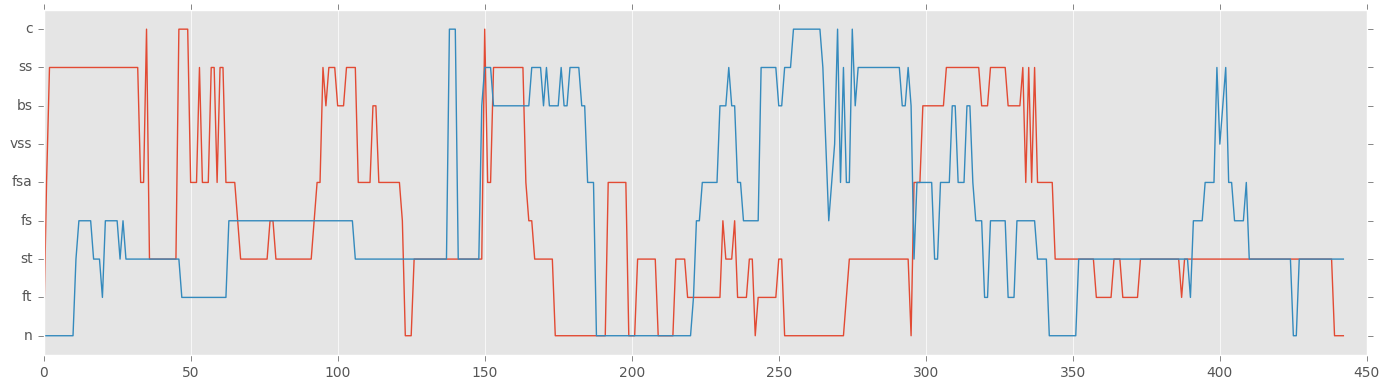
\includegraphics[width=\textwidth]{duo-test-1}
  \caption{A generated duet with one lead performer (shown in red)
    taken from a real performance and an ANN-generated duo partner
    (shown in blue).}\label{fig:duo-model}
\end{figure}

The simplest ensemble configuration is a duet between two performers.
In this model, the input for the network is the current gesture of the
lead performer and the previous gesture of the second player while the
output is the current gesture of the other player. Training data was
constructed by taking each performer as leader and constructing
examples for each other player present in the performance. All
ensemble performances from the corpus were treated in this manner and
each sequence of 120 states was taken as a separate training example
resulting in a total of 319948 examples.

Figure \ref{fig:duo-model} shows an example output from the network
with a lead player taken from a real performance shown in red and a
generated duo partner shown in blue. The generated player shows a
similar complexity to the lead player and appears to mimic the
leader's gestures at some points in what, when sonified, could be a
convincing duet performance.



\subsection{Quartet}

Performances with four players were the most numerous ensemble
configuration in the corpus. In this model the input for the network
was the current gesture of lead player and previous gesture of the
three other players. The output was the predicted gestures for the
three others in the group.

\begin{figure}
  \centering
  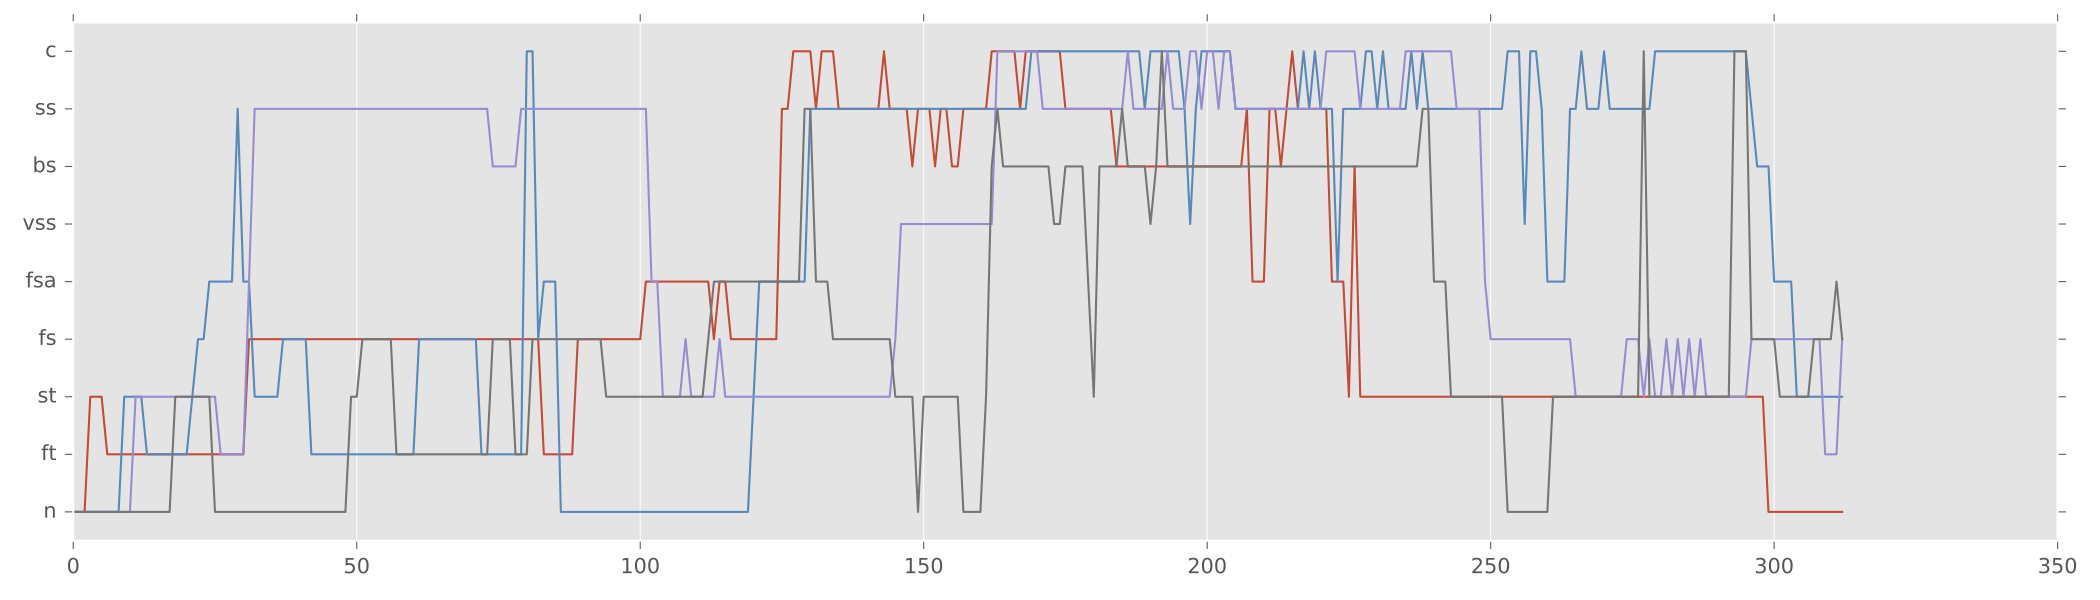
\includegraphics[width=\textwidth]{quartet-performance-512nodes-16}
  \caption{An example performance using the quartet model network. The
    lead performer is shown in red and three other performers were
    generated by the ANN. These results show some realistic ensemble
    interaction and suggest that this model might be useful for
    practical applications.}\label{fig:quartet-model}
\end{figure}

Training data was constructed similarly to the duet model, with each
performer in the group considered as a lead player. As the ordering of
the other three players was significant in the encoding (but not in
the actual performance), a separate training example was constructed
for each permutation of the other players in the ensemble.

The quartet model ANN was trained on the whole dataset of quartet
performances. This dataset consisted of 33 performances with total
length of 5.28 hours corresponding to 19023 gesture state
measurements. The ANN was trained for 30 epochs using mini-batches of
64 performance examples; training time was 9.42 hours.

An example of a generated ensemble performance is shown in Figure
\ref{fig:quartet-model}. In this figure, the red line shows a real
gesture state sequence taken from a non-quartet improvisation (not
used to train the ANN), and the other three lines show generated state
sequences primed with the ``nothing'' gesture in the first state. From
this and other generated examples, the ANN appears to be sufficiently
capable of generating ensemble parts to warrant further investigation.

\section{Conclusions and Future Work}

This paper reports on work-in-progress towards a practical ANN model
of ensemble interaction for touch-screen performances. So far,
recurrent neural networks with LSTM cells have been implemented and
trained to generate duets and quartets in response to a single lead
player. While visualising the results suggests that realistic ensemble
interactions are being generated, further work needs to be done to
clearly that the ensemble generations are accurate and demonstrate
more interesting interactions than unrelated sequences. However, based
on the current results, it may be most interesting to implement
sonifications of the generated gesture sequences so that they can be
used in real-time performance as a computer accompaniment to a live
touch-screen performer.

\subsubsection*{Acknowledgments}
This work is partially supported by The Research Council of Norway as
a part of the Engineering Predictability with Embodied Cognition
(EPEC) project, under grant agreement 240862.

\bibliographystyle{SIGCHI-Reference-Format}
\bibliography{2013ComputerMusic}

\end{document}
